\chapter{The Downside Floor}

This short School of Hard Knocks interview segment, curated by LazyingArt LLC through Video2Book, gives us a compact but useful piece of entrepreneurial reasoning. The question is not whether risk is glamorous. The question is how a founder decides whether a risk is actually survivable. The speaker answers by putting a floor under the downside: if the attempt failed, he could still get a job. From there, the calculation changes. The danger is no longer only business failure. The danger is also the future cost of never trying.

\section{Risk As A Career Pattern}

The interviewer does not ask for one spectacular moment. He asks how important risk was throughout the speaker's career, and then broadens the question: not just one instance, but the general act of taking risks.

That opening matters. We should not read the answer as a single dramatic story. The speaker is describing a working rule, a way of judging uncertain decisions. In these notes, we can write the basic setup as two possible choices:
\begin{equation}
T = \text{try the venture},
\qquad
N = \text{do not try}.
\end{equation}
This notation is only a bookkeeping device for the chapter. The interview gives us the logic in ordinary language, not as a formal model.

\section{The Downside Floor}

The speaker begins with his risk mentality ``at the time.'' The first move is not to estimate an upside. It is to name the worst credible downside. In his words, the worst thing that could happen was that he would have to get a job.

Let
\[
F = \text{failure},
\qquad
J = \text{job fallback}.
\]
The transcript-backed relation is then:
\begin{equation}
F \longrightarrow J.
\end{equation}
That is the entire mechanism of the answer. Failure is not described as pleasant, profitable, or costless. It is described as recoverable. The job is the fallback state, and the existence of that fallback changes the meaning of risk.

\begin{definition}
A \emph{downside floor} is the practical lower bound a founder assigns to a risk. In this interview, the downside floor is not bankruptcy, exile, or permanent ruin. It is returning to employment.
\end{definition}

This is why the answer is stronger than a slogan about courage. The speaker is not saying, ``ignore the downside.'' He is saying, in effect, ``define the downside honestly, and then decide whether it is survivable.''

\section{Responsibility Enters The Calculation}

The next detail is important: he had a newborn on the way. That phrase raises the emotional and practical stakes. If we omit it, the argument becomes too easy. A risk taken with no dependents is one kind of decision; a risk taken while a child is coming is another.

We can mark this contextual pressure as a constraint:
\begin{equation}
K = \text{family responsibility}.
\end{equation}
The interview does not quantify \(K\), and we should not pretend that it does. But it changes the interpretation. The point is not that responsibility disappears. The point is that responsibility makes the fallback more important. With a newborn on the way, the question becomes sharper:
\[
\text{Is the failure path still recoverable?}
\]
For the speaker, the answer was yes, because the failure path returned to work.

\section{The Real Risk}

After defining the downside, the speaker moves to action: let me take the risk. The order is worth preserving. He does not first announce a heroic appetite for risk and then justify it later. He first bounds the loss, then allows himself to act.

\subsection{Question \& Answer}

\paragraph{Question.}
Was the real risk simply that the venture might fail?

\paragraph{Answer.}
Not in the speaker's own framing. Venture failure was one risk, but he treated it as recoverable because failure led back to employment:
\begin{equation}
T \ \text{and then} \ F \longrightarrow J.
\end{equation}
The more durable risk was different. If he did not try, he imagined himself sitting at a job later, asking why he never attempted it. So the path of inaction also returns to employment, but with an added cost:
\begin{equation}
N \longrightarrow J + R_N,
\end{equation}
where \(R_N\) denotes the regret or counterfactual burden of not trying.

This is not a formula quoted from the speaker. It is a compact reconstruction of the comparison he makes in the interview.

\section{A Small Decision Derivation}

We can now write the speaker's practical comparison in a deliberately simple form. Let \(C_T\) be the personal cost of trying and failing, and let \(C_N\) be the personal cost of not trying. The transcript supports the following qualitative structure:
\begin{align}
C_T &\approx D_J, \\
C_N &\approx D_J + R_N,
\end{align}
where \(D_J\) is the burden of returning to a job and \(R_N\) is the lasting regret of never trying.

Subtract the two:
\begin{align}
C_N - C_T
&\approx (D_J + R_N) - D_J \\
&= R_N.
\end{align}
So, under the speaker's own simplified comparison, if the regret of not trying is real and persistent, then:
\begin{equation}
R_N > 0
\qquad \Longrightarrow \qquad
C_N > C_T.
\end{equation}
This is the mathematical skeleton of the passage. The job fallback appears on both sides of the comparison. Trying and failing may put him back in a job; not trying leaves him in a job too. The difference is that the no-try path carries the extra weight of wondering why he never made the attempt.

\begin{figure}
\centering
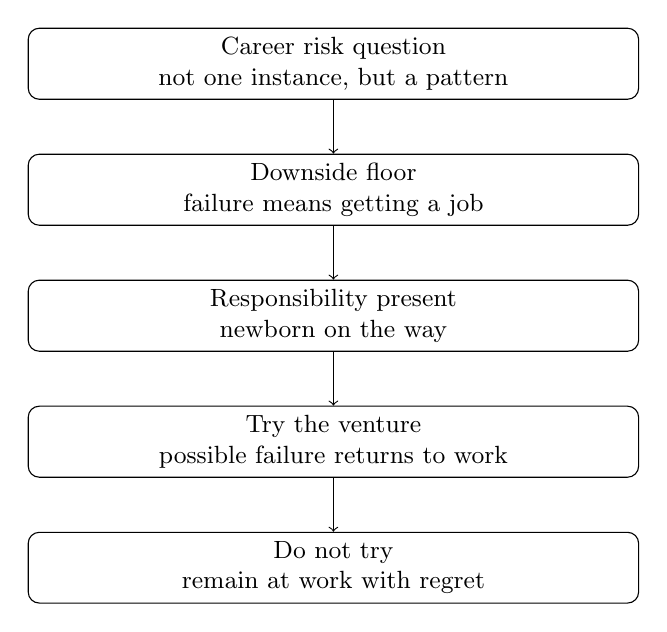
\begin{tikzpicture}[every node/.style={font=\small}]
\node[draw, rounded corners, align=center, text width=0.62\linewidth] (q) at (0,0)
{Career risk question\\not one instance, but a pattern};

\node[draw, rounded corners, align=center, text width=0.62\linewidth] (floor) at (0,-1.6)
{Downside floor\\failure means getting a job};

\node[draw, rounded corners, align=center, text width=0.62\linewidth] (responsibility) at (0,-3.2)
{Responsibility present\\newborn on the way};

\node[draw, rounded corners, align=center, text width=0.62\linewidth] (try) at (0,-4.8)
{Try the venture\\possible failure returns to work};

\node[draw, rounded corners, align=center, text width=0.62\linewidth] (nottry) at (0,-6.4)
{Do not try\\remain at work with regret};

\draw[->] (q) -- (floor);
\draw[->] (floor) -- (responsibility);
\draw[->] (responsibility) -- (try);
\draw[->] (try) -- (nottry);
\end{tikzpicture}
\caption{A transcript-derived decision schematic. The visual is a reconstruction of the speaker's reasoning, not a board diagram from the video.}
\end{figure}

\section{The Cost Of Not Trying}

The closing move in the excerpt is the most important one. The speaker says that if he did not try, he would be sitting at a job someplace, always wondering why he had not attempted it.

That turns the chapter from risk into opportunity cost. The obvious risk is the failed venture. The less obvious risk is the permanent counterfactual. A job appears in both outcomes, but it has a different meaning in each:
\begin{align}
\text{failure after trying} &\longrightarrow \text{job as fallback}, \\
\text{never trying} &\longrightarrow \text{job as regret site}.
\end{align}
This is the entrepreneurial distinction the interview contributes to the larger book. A founder does not only ask, ``What happens if this fails?'' The founder also asks, ``What happens to me if I never test it?''

\section{Summary}

The lecture segment gives us a tight decision principle. First, define the downside. Second, ask whether that downside is survivable. Third, include the real pressures around the decision, such as family responsibility. Fourth, compare failure with inaction, not with an imaginary risk-free life.

For this speaker, the fallback was employment. That made failure recoverable. But not trying carried its own cost: sitting in a job later and wondering why he had not taken the risk. The practical lesson is not to take every risk. It is to distinguish a recoverable downside from a regret that may last much longer.